%% generato automaticamente da tools/build_tex.py --- non modificare
\chapter{Una somma sola}
\label{cap:numeri-primi}
\quaderno{numeri primi.dfw}{27 Aug 2010}{1}

Agosto 2010, lo stesso giorno di \dfw{pigreco.dfw}. Il file contiene una sola espressione, lunga 573 caratteri: la somma dei reciproci dei primi diciannove primoriali, scritta per esteso, con tutti i denominatori sviluppati come prodotti di numeri primi.

È anche il file che, durante il recupero, per un po' è sembrato vuoto. Il formato \dfw{.dfw} memorizza la lunghezza del testo in un byte, e un byte arriva a 254: le espressioni più lunghe usano una codifica estesa che il primo estrattore non riconosceva. Vedere \dfw{numeri primi.dfw} passare da zero a una espressione è stato il segnale che quella codifica esisteva.

\section{La somma}
\begin{espr}{1}{User}{}
\begin{align*}
& \frac{1}{2} + \frac{1}{2 \cdot 3} + \frac{1}{2 \cdot 3\, 5} + \frac{1}{2 \cdot 3\, 5\, 7} + \frac{1}{2 \cdot 3\, 5\, 7\, 11} + \frac{1}{2 \cdot 3\, 5\, 7\, 11\, 13} \\
&\qquad + \frac{1}{2 \cdot 3\, 5\, 7\, 11\, 13\, 17} + \frac{1}{2 \cdot 3\, 5\, 7\, 11\, 13\, 17\, 19} + \frac{1}{2 \cdot 3\, 5\, 7\, 11\, 13\, 17\, 19\, 23} + \frac{1}{2 \cdot 3\, 5\, 7\, 11\, 13\, 17\, 19\, 23\, 29} \\
&\qquad + \frac{1}{2 \cdot 3\, 5\, 7\, 11\, 13\, 17\, 19\, 23\, 29\, 31} + \frac{1}{2 \cdot 3\, 5\, 7\, 11\, 13\, 17\, 19\, 23\, 29\, 31\, 37} + \frac{1}{2 \cdot 3\, 5\, 7\, 11\, 13\, 17\, 19\, 23\, 29\, 31\, 37\, 41} \\
&\qquad + \frac{1}{2 \cdot 3\, 5\, 7\, 11\, 13\, 17\, 19\, 23\, 29\, 31\, 37\, 41\, 43} + \frac{1}{2 \cdot 3\, 5\, 7\, 11\, 13\, 17\, 19\, 23\, 29\, 31\, 37\, 41\, 43\, 47} \\
&\qquad + \frac{1}{2 \cdot 3\, 5\, 7\, 11\, 13\, 17\, 19\, 23\, 29\, 31\, 37\, 41\, 43\, 47\, 53} + \frac{1}{2 \cdot 3\, 5\, 7\, 11\, 13\, 17\, 19\, 23\, 29\, 31\, 37\, 41\, 43\, 47\, 53\, 59} \\
&\qquad + \frac{1}{2 \cdot 3\, 5\, 7\, 11\, 13\, 17\, 19\, 23\, 29\, 31\, 37\, 41\, 43\, 47\, 53\, 59\, 61} + \frac{1}{2 \cdot 3\, 5\, 7\, 11\, 13\, 17\, 19\, 23\, 29\, 31\, 37\, 41\, 43\, 47\, 53\, 59\, 61\, 67}
\end{align*}
\end{espr}
Diciannove termini, dal reciproco di $2$ al reciproco del primoriale di $67$. Ogni denominatore è il precedente moltiplicato per il primo successivo.

\begin{figure}[htbp]
  \centering
  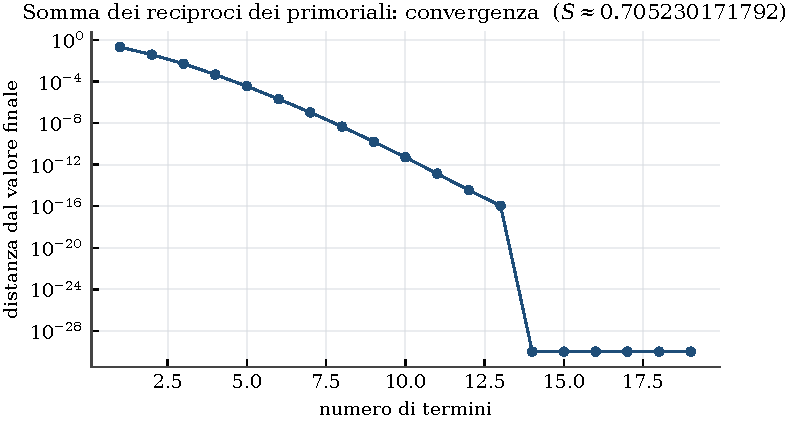
\includegraphics[width=0.86\linewidth]{../figures/primoriale.pdf}
  \caption{Distanza fra le somme parziali e il valore finale, in scala logaritmica. La convergenza è più che geometrica: ogni termine aggiunge almeno una cifra corretta, e negli ultimi passi molte di più.}
  \label{fig:primoriale}
\end{figure}

Il primoriale di $p$ è il prodotto di tutti i primi minori o uguali a $p$: $2$, poi $6$, poi $30$, $210$, $2310$, e così via. La somma dei loro reciproci converge molto rapidamente, perché ogni denominatore è almeno il doppio del precedente. I diciannove termini scritti nel quaderno — fino al primoriale di $67$, che ha venticinque cifre — danno
\[
  \sum_{n\ge1}\frac{1}{p_n\#}=0{,}70523017179180096\ldots
\]
e le cifre riportate sono già tutte quelle che i diciannove termini determinano: il ventesimo termine è dell'ordine di $10^{-27}$.

Il numero non ha una forma chiusa nota. È irrazionale — lo si dimostra con lo stesso argomento che vale per $\mathrm{e}$, perché la coda della serie dopo il termine $n$-esimo è più piccola del termine stesso — ma non se ne conosce altro. Il quaderno non aggiunge commenti, e in questo caso è comprensibile: era il posto dove annotare il valore, non dove studiarlo.

Vale la pena osservare come è scritta l'espressione. I denominatori non sono $2$, $6$, $30$, $210$: sono $2$, $2\cdot3$, $2\cdot3\cdot5$, $2\cdot3\cdot5\cdot7$. La struttura del primoriale è lasciata visibile, e la somma si legge come un elenco di primi che si allunga di uno a ogni riga.

